\chapter{Rezepte: durchgerechnete Beispiele}\label{ch:rezepte}

Jedes Rezept nennt die Aufgabe, die Konfiguration, das Ergebnis und worauf zu achten ist. Alle Zahlen sind mit
\FG{} 0.18 auf einem Rechner mit zwei Kernen gerechnet.

%-------------------------------------------------------------------------------------------
\section{Antireflexschicht}
\index{Antireflexschicht}%
\textbf{Aufgabe:} Eine $\lambda/4$-Schicht MgF$_2$ ($n=1{,}38$) auf Glas ($n=1{,}52$) für 550\,nm. Wie stark
reflektiert die Oberfläche?
\begin{lstlisting}[language=json]
{ "dimension": "1D", "solver": "rcwa", "truncation": { "Nx": 0 }, "period_um": { "x": 1.0 },
  "incidence": { "lambda_um": [0.45, 0.55, 0.65], "phi_deg": 0, "delta_deg": 0 },
  "materials": { "air": {"n": 1.0}, "glass": {"n": 1.52}, "mgf2": {"n": 1.38} },
  "superstrate": "air", "substrate": "glass",
  "layers": [ { "type": "homogeneous", "thickness_um": 0.09964, "material": "mgf2" } ] }
\end{lstlisting}
\textbf{Ergebnis:} $R=1{,}62\,\%$ (450\,nm), $1{,}26\,\%$ (550\,nm), $1{,}44\,\%$ (650\,nm). Die analytische Formel
$R=\bigl((n_s-n^2)/(n_s+n^2)\bigr)^2=1{,}26\,\%$ wird exakt getroffen; ohne Schicht wären es 4,26\,\%.

\textbf{Worauf achten:} Ohne Gitter genügt $N_x=0$; die Periode ist dann beliebig. Für einen Schichtstapel fügen Sie
weitere \val{homogeneous}-Schichten an.

%-------------------------------------------------------------------------------------------
\section{Dielektrisches Transmissionsgitter: beide Polarisationen}
\textbf{Aufgabe:} Das Lamellengitter aus Kapitel~\ref{ch:schnellstart} über 0,5--0,8\um, s und p, und die Effizienz
für unpolarisiertes Licht.
\begin{lstlisting}[style=py]
cfg = fg.load_config("examples/v3_lamellar_dielectric.json")
cfg["incidence"]["lambda_um"] = {"from": 0.5, "to": 0.8, "steps": 61}
cfg["incidence"]["delta_deg"] = [0, 90]
c = fg.solve_scan(cfg).columns
for pol in (0, 90):
    sel = (c["side"] == "T") & (c["n"] == 1) & (c["delta_deg"] == pol)
    print(pol, c["efficiency"][sel].max())
\end{lstlisting}
\textbf{Worauf achten:} Für dielektrische Lamellen ist $N=15$ ausreichend; die Energiebilanz ist exakt 1. Die
Mittelung $\tfrac12(e_s+e_p)$ ergibt unpolarisiertes Licht.

%-------------------------------------------------------------------------------------------
\section{Gold-Echelette: Winkel-Scan mit RK}
\textbf{Aufgabe:} Ein Dreieckgitter in Gold (Periode 1\um, Tiefe 0,25\um, Spitze bei 0,7\um), TM, 633\,nm,
Einfallswinkel 10--40$^\circ$. Wie viel Licht geht in die Ordnung $-1$?
\begin{lstlisting}[language=json]
{ "dimension": "1D", "solver": "rk", "truncation": { "Nx": 12 }, "period_um": { "x": 1.0 },
  "incidence": { "lambda_um": 0.6328, "phi_deg": { "from": 10, "to": 40, "steps": 4 },
                 "delta_deg": 90 },
  "materials": { "air": {"n": 1.0}, "au": {"n": [0.2, 3.4]} },
  "superstrate": "air", "substrate": "au",
  "layers": [ { "type": "profile1d", "shape": "triangle", "depth_um": 0.25, "apex_x_um": 0.7,
                "below": "au", "above": "air" } ],
  "rk": { "tableau": "gauss2", "tol": 1e-5 } }
\end{lstlisting}
\textbf{Ergebnis} (\file{examples/echelette\_au\_scan.json}, 28\,s):
\begin{center}
\small
\begin{tabular}{rcccc}
\toprule
$\varphi$ & $R_{-2}$ & $R_{-1}$ & $R_0$ & Absorption \\
\midrule
10° & -- & 0,447 & 0,148 & 0,133 \\
20° & 0,046 & 0,674 & 0,069 & 0,097 \\
30° & 0,191 & 0,546 & 0,028 & 0,235 \\
40° & 0,145 & 0,630 & 0,060 & 0,165 \\
\bottomrule
\end{tabular}
\end{center}
\textbf{Worauf achten:} Das Substrat absorbiert, also gibt es keine transmittierten Ordnungen. Das Dreieck hat Ecken;
\val{auto} wählt \val{FFF\_sym}. Für Endergebnisse $N$ auf 20--30 erhöhen und \key{rk.tol} auf $10^{-7}$ senken. Der
Referenzfall V14 zeigt, dass Dreiecksgitter in Gold in TM keine leichte Aufgabe sind.

%-------------------------------------------------------------------------------------------
\section{Metallgitter in TM mit ASR}
\textbf{Aufgabe:} Goldlamellen in TM genau rechnen (Referenzfall V19). Ohne Maßnahmen konvergiert $e_{-1}$ sehr
langsam (Abschnitt~\ref{sec:konvergenz}).
\begin{lstlisting}[language=json]
"layers": [ { "type": "lamellar1d", "thickness_um": 0.3, "breakpoints_um": [0, 0.5, 1.0],
              "materials": ["au", "air"] } ],
"coordinate_transform": { "x": { "type": "asr", "eta": 0.95, "breakpoints_um": "auto" } },
"truncation": { "Nx": 20 }
\end{lstlisting}
\textbf{Ergebnis:} $e_{-1}=0{,}01358$, $e_0=0{,}79421$ bei $N=20$; der Grenzwert ist $0{,}013591$ bzw.\ $0{,}79435$.
Ohne ASR liegt $e_{-1}$ bei $N=80$ noch bei $0{,}01346$.

%-------------------------------------------------------------------------------------------
\section{Siliziumsäulen: 2D-Gitter mit Nahfeld}
\textbf{Aufgabe:} Quadratische Siliziumsäulen (0,3\um{} breit, 0,15\um{} hoch, Periode 0,6\um) auf Glas; Effizienzen
und Feld in halber Höhe.
\begin{lstlisting}[language=json]
{ "dimension": "2D", "solver": "rcwa", "truncation": { "Nx": 4, "Nz": 4 },
  "period_um": { "x": 0.6, "z": 0.6 },
  "incidence": { "lambda_um": 0.6328, "phi_deg": 10, "psi_deg": 0, "delta_deg": 90 },
  "materials": { "air": {"n": 1.0}, "glass": {"n": 1.5}, "si": {"n": [3.88, 0.02]} },
  "superstrate": "air", "substrate": "glass",
  "layers": [ { "type": "polygon2d", "thickness_um": 0.15, "background": "air",
                "inclusions": [ { "material": "si",
                  "rectangle_um": { "center": [0.3, 0.3], "size": [0.3, 0.3] } } ] } ],
  "nearfield": { "enabled": true, "horizontal_y_um": 0.075, "vertical_z_um": 0.3,
                 "y_range_um": [-0.2, 0.35], "nx": 120, "ny": 110, "nz": 120, "periods": 2 } }
\end{lstlisting}
\textbf{Ergebnis} (\file{examples/nearfield\_pillars\_2d.json}, 1,7\,s): $R_{-1,0}=0{,}233$, $R_{0,0}=0{,}090$, sieben
transmittierte Ordnungen, Absorption 21\,\%. Die Ordnungen $(n,\pm1)$ sind gleich stark -- die Struktur ist
spiegelsymmetrisch in $z$ und $\psi=0$. Das Nahfeld zeigt Kapitel~\ref{ch:nahfeld}.

\textbf{Worauf achten:} $N=4$ ist eine Übersicht. Für Endergebnisse $N=6$ und $N=8$ vergleichen (Rechenzeit
wächst etwa um den Faktor 9 bzw.\ 45).

%-------------------------------------------------------------------------------------------
\section{Silber-Lochgitter: Spektrum mit Plasmonenresonanz}\label{sec:rez-loch}
\index{Lochgitter}\index{Plasmonenresonanz}%
\textbf{Aufgabe:} Ein Silberfilm (0,2\um) auf Glas mit quadratischen Löchern (0,25\um, Periode 0,9\um), senkrechter
Einfall: außergewöhnliche Transmission (Referenzfall V10).
\begin{lstlisting}[language=json]
{ "dimension": "2D", "solver": "rcwa", "truncation": { "Nx": 6, "Nz": 6 },
  "period_um": { "x": 0.9, "z": 0.9 },
  "incidence": { "lambda_um": { "from": 1.30, "to": 1.50, "steps": 41 },
                 "phi_deg": 0, "psi_deg": 180, "delta_deg": 0 },
  "materials": { "air": {"n": 1.0}, "glass": {"n": 1.5}, "ag": {"n": [0.1, 8.94]} },
  "superstrate": "air", "substrate": "glass",
  "layers": [ { "type": "polygon2d", "thickness_um": 0.2, "background": "ag",
                "inclusions": [ { "material": "air",
                  "vertices_um": [[0.325,0.325],[0.575,0.325],[0.575,0.575],[0.325,0.575]] } ] } ] }
\end{lstlisting}
\textbf{Ergebnis} (41 Wellenlängen, 58\,s): Die Transmission ist fast überall unter 0,5\,\%, steigt aber knapp oberhalb
der Plasmonenresonanz der ebenen Grenzfläche ($\lambda=1{,}3694$\um) auf 3,0\,\% bei $\lambda=1{,}385$\um{} -- rund dreißigmal so viel wie bei 1,5\um{}
(0,10\,\%), obwohl die Löcher mit 0,25\um{} Kantenlänge viel kleiner als die Wellenlänge sind. Gleichzeitig steigt die
Absorption von 2\,\% auf 10\,\%. Das Buch nennt $T\approx7{,}5\,\%$ bei 1,388\um; bei $N=6$ ist der Peak noch nicht
konvergiert.
\begin{figure}[h]
\centering
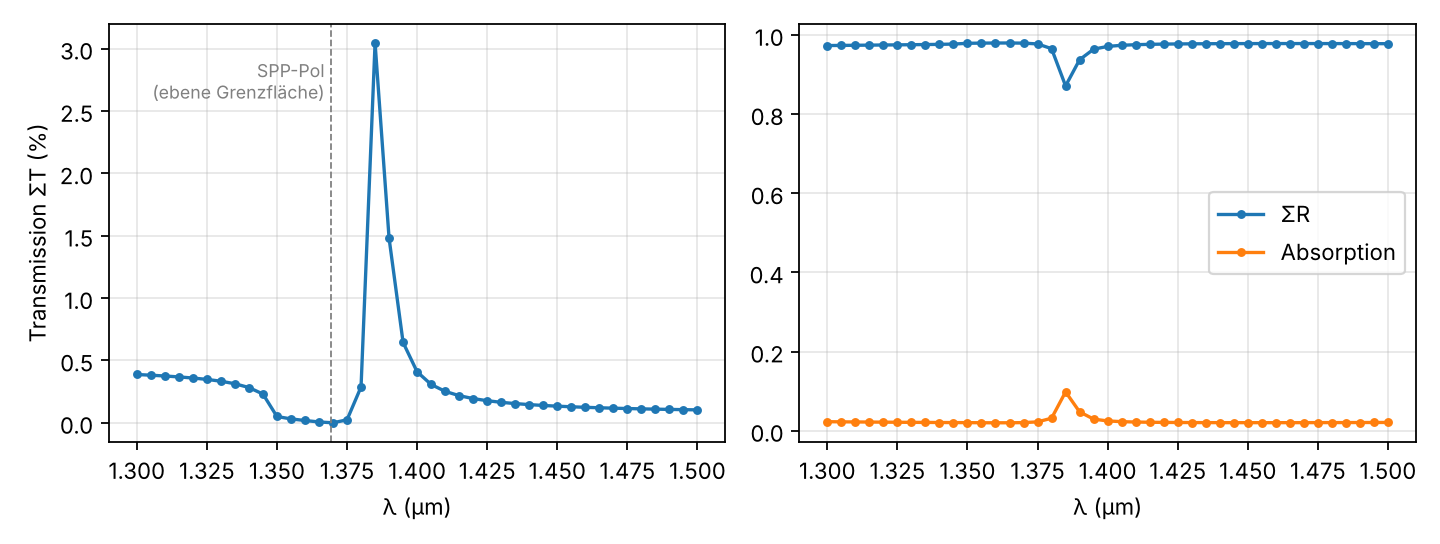
\includegraphics[width=\linewidth]{fig/v10_spec.png}
\caption{Silber-Lochgitter, $N_x=N_z=6$: Transmission (links), Reflexion und Absorption (rechts). Gestrichelt: Pol
des Oberflächenplasmons an der ebenen Silber-Luft-Grenzfläche.}
\end{figure}

\textbf{Worauf achten:} Die Brechzahl von Silber ist hier für alle Wellenlängen gleich, wie im Referenzfall des
Buchs. Für quantitative Spektren ein dispersives Modell oder eine Tabelle einsetzen
(Abschnitt~\ref{sec:conf-dispersion}), z.\,B.\ das Drude--Lorentz-Modell aus
\file{examples/dispersive\_metal\_grating.json}. Die Lage des Peaks verschiebt sich mit $N$; Spektren für $N=6,8,10$
vergleichen.

%-------------------------------------------------------------------------------------------
\section{Einzelner Steg mit PML}
\textbf{Aufgabe:} Ein Siliziumsteg (0,3\um{} breit, 0,2\um{} hoch) auf Glas. Wie viel Licht streut er?
\begin{lstlisting}[language=json]
{ "dimension": "1D", "solver": "rcwa", "truncation": { "Nx": 60 }, "period_um": { "x": 4.0 },
  "incidence": { "lambda_um": 0.6328, "phi_deg": 0, "delta_deg": 0 },
  "materials": { "air": {"n": 1.0}, "glass": {"n": 1.5}, "si": {"n": [3.88, 0.02]} },
  "superstrate": "air", "substrate": "glass",
  "layers": [ { "type": "lamellar1d", "thickness_um": 0.2,
                "breakpoints_um": [0, 1.85, 2.15, 4.0], "materials": ["air", "si", "air"] } ],
  "aperiodic": { "pml": { "x": { "width_um": 0.8, "beta": 1.0 } } } }
\end{lstlisting}
\textbf{Ergebnis} (8\,s): Streubreite nach oben 0,329\um, nach unten 0,370\um, absorbiert 0,023\um. Bei
$\varphi=20^\circ$ (automatisch Streufeldformulierung): 0,340 / 0,345 / 0,042\um.

\textbf{Worauf achten:} Zellbreite und $N$ gemeinsam erhöhen und prüfen, dass die Summe stabil ist. Die Struktur
muss vollständig im physikalischen Bereich $[0{,}8;\,3{,}2]$\um{} liegen.

%-------------------------------------------------------------------------------------------
\section{Säule unter einem Gauß-Strahl (Zylinder)}
\textbf{Aufgabe:} Eine SiN-Säule ($n=1{,}45$, Radius 0,4\um, Höhe 0,3\um) auf Glas, beleuchtet von einem fokussierten
Gauß-Strahl (Taille 0,5\um), 0,9--1,1\um.

\textbf{Konfiguration:} \file{examples/cyl\_pillar\_beam.json} (Abschnitt~\ref{sec:zylinder}).

\textbf{Ergebnis} (14\,s für drei Wellenlängen): Bei 0,9\um{} werden 4,74\,\% reflektiert und 95,24\,\% transmittiert,
je zur Hälfte in den Harmonischen $m=\pm1$ (x-Polarisation). \texttt{C\_A} liegt zwischen $-1{,}7\cdot10^{-4}$ und
$1{,}2\cdot10^{-4}$ -- bei verlustfreien Materialien ein Maß für die Genauigkeit des Spektrums; \key{kappa\_max}
erhöhen, wenn mehr nötig ist.

%-------------------------------------------------------------------------------------------
\section{Freiform-Profil mit Hinterschnitt als NURBS}
\index{NURBS}\index{Ueberhang@Überhang}\index{Schichttyp!profile1d@\texttt{profile1d}!nurbs@\texttt{nurbs}}%
\textbf{Aufgabe:} Eine Lackline mit überhängendem Kopf („Pilz“, Periode 0,3\um) auf Silizium, TM, 633\,nm unter
$10^\circ$. Wie viel wird reflektiert? Als Funktion $y=g(x)$ geht das nicht, eine STEP-Datei ist nicht nötig.
\begin{lstlisting}[language=json]
{ "dimension": "1D", "solver": "rk", "truncation": { "Nx": 15 }, "period_um": { "x": 0.3 },
  "incidence": { "lambda_um": 0.633, "phi_deg": 10, "psi_deg": 0, "delta_deg": 90 },
  "materials": { "air": {"n": 1.0}, "resist": {"n": 1.6}, "si": {"n": [3.88, 0.02]} },
  "superstrate": "air", "substrate": "si", "rk": { "tol": 1e-8 },
  "layers": [ { "type": "profile1d", "shape": "nurbs", "below": "resist", "above": "air",
    "nurbs": { "degree": 2, "knots": [0,0,0, 1,1, 2,2, 3,3, 4,4, 5,5, 6,6, 7,7,7],
      "points_um": [[0.0, 0.02], [0.065, 0.02], [0.13, 0.02], [0.14, 0.06], [0.12, 0.09],
                    [0.05, 0.10], [0.08, 0.13], [0.15, 0.19], [0.22, 0.13], [0.25, 0.10],
                    [0.18, 0.09], [0.16, 0.06], [0.17, 0.02], [0.235, 0.02], [0.3, 0.02]] } } ] }
\end{lstlisting}
Die Kurve besteht aus sieben quadratischen Bézierstücken (innere Knoten doppelt): Restschicht, Stiel links, Kopf
links (nach außen, der Überhang), Kopf oben, Kopf rechts, Stiel rechts, Restschicht. Sie beginnt bei $(0;\,0{,}02)$
und endet eine Periode weiter auf derselben Höhe.

\textbf{Ergebnis:} $R_0=0{,}25484$ (RK, 23\,s); RCWA mit 80 Scheiben liefert dasselbe auf $3\cdot10^{-6}$ in 3\,s.

\textbf{Worauf achten:} Die Linie läuft insgesamt von links nach rechts, \key{below} liegt darunter. Die Höhe der
Schicht ist ohne \key{depth\_um} die Oberkante der Kurve (hier 0,16\um). Ein Fehler wie
\texttt{/layers/0: [NURBS\_PERIOD]} heißt: der letzte Punkt liegt nicht genau eine Periode rechts vom ersten.
Selbstschnitte (auch mit dem Nachbarn der nächsten Periode) meldet \texttt{NURBS\_SELF\_INTERSECTION}.

%-------------------------------------------------------------------------------------------
\section{Littrow-Gitter optimieren}
\index{Littrow}%
\textbf{Aufgabe:} Ein Aluminium-Lamellengitter (Periode 0,5\um, TM) so auslegen, dass möglichst viel Licht in die
Ordnung $-1$ zurückgeht.

\textbf{Lösung:} \file{examples/python/optimize\_littrow.py} oder in der GUI \gui{Optimierung} $\to$
\gui{Littrow-Vorlage laden}. Parameter sind Tiefe (\val{/layers/0/thickness\_um}) und Stegbreite
(\val{/layers/0/breakpoints\_um/1}). Das Skript vergleicht das Ergebnis von L-BFGS-B mit einem Rasterscan; jede
Auswertung mit Gradient kostet nur etwa 1,3--2,5 Vorwärtsrechnungen, unabhängig von der Zahl der Parameter.

%-------------------------------------------------------------------------------------------
\section{Konvergenzstudie als Sweep}
\index{Konvergenz!Studie}%
\begin{lstlisting}[language=json]
"sweep": { "parameter": "/truncation/Nx", "values": [10, 20, 40, 80] }
\end{lstlisting}
Mit \file{plot\_efficiencies.py \ldots{} --x sweep\_value} entsteht direkt die Konvergenzkurve. In 2D müssen $N_x$ und
$N_z$ gemeinsam wachsen; dafür eine Python-Schleife verwenden.
